% ============================================================
%  Experiment 4 --- LCD Interfacing to Altera DE2 Board, and
%  Stepper Motor Control with FPGA
%  (merged from the former Experiment 5 and Experiment 6)
% ============================================================
\experimentheader{4}{Experiment 4}{LCD Interfacing to Altera DE2 Board, and Stepper Motor Control with FPGA}{FPGA Lab}

\begin{objectives}
  \begin{enumerate}
    \item To use Verilog code as a design entry method in Altera Quartus II Software.
    \item To interface an LCD module to the Altera DE2 board.
    \item To design digital circuits in an FPGA to control a stepper motor.
    \item To simulate the circuit using Altera Quartus II Software.
    \item To download the design onto an Altera DE2 board.
  \end{enumerate}
\end{objectives}

\begin{equipment}
  \begin{enumerate}
    \item Altera Quartus II software
          \begin{itemize}
            \item version 9/10/12 for Cyclone II
            \item version 9/10/12/latest for Cyclone IV
          \end{itemize}
    \item Altera DE2 board
    \item Parallax 4-phase, 12\,V, 75\,$\Omega$ unipolar stepper motor
    \item ULN2003 Darlington transistor array (motor driver)
  \end{enumerate}
\end{equipment}

\begin{introduction}
  In recent years, LCDs have largely replaced simple LED displays: they can show numbers, characters, and graphics, and are relatively easy to program. Table~\ref{tab:exp5-pins-lcd} lists the LCD pins relevant to programming.
  \vspace*{10pt}

  The \textit{enable} (E) pin is used by the LCD to latch the information presented on its data pins: a high-to-low transition on E must be applied for the LCD to latch the data, and this pulse must be at least 450\,ns wide. The required timing is shown in Figure~\ref{fig:exp5-timing}.
  \vspace*{10pt}

  Two important internal registers are selected via the RS pin. When $\text{RS}=0$, the \textit{instruction/command} register is selected, allowing commands to be sent to the LCD (Table~\ref{tab:exp5-commands} lists the available command codes). When $\text{RS}=1$, the \textit{data} register is selected, allowing ASCII character data to be written for display, sent through data pins D0--D7.
  \vspace*{10pt}

  It is good practice to check the busy flag before writing to the LCD: with $\text{RS}=0$ and $\text{R}/\overline{\text{W}}=1$, the busy flag appears on D7. While D7\,=\,1 the LCD is busy with internal operations and will not accept new data; once D7\,=\,0, the LCD is ready to receive the next byte.
  \vspace*{10pt}

  Unlike an ordinary DC motor, a stepper motor does not spin freely when power is applied --- it must be driven with a continuously pulsed sequence of specific coil-energising patterns. Each pulse advances the rotor by a fixed step angle (for this motor, $3.6^\circ$ per step), which is what gives stepper motors their positioning precision: as long as speed and torque stay within the motor's limits, the controller always knows the rotor's exact position.
  \vspace*{1.5em}

  The rotor is driven by the interaction of magnetic fields as coils are switched on and off in sequence. Table~\ref{tab:exp6-stepseq} shows the normal four-coil unipolar step sequence; taking a step means driving two of the four coil-driver pins high at a time, in the order shown, through the ULN2003 driver.
\end{introduction}

\needspace{4cm}
\begin{boxedtable}
  \captionof{table}{Pin description for the LCD module.}
  \label{tab:exp5-pins-lcd}
  {\renewcommand{\arraystretch}{1.5}
    \centering
    \begin{tabular}{cccc}
      \toprule
      Pin & Symbol                  & I/O & Description                                                                                                                    \\
      \midrule
      1   & $V_{ss}$                & --- & Ground                                                                                                                         \\
      2   & $V_{cc}$                & --- & $+5\,\text{V}$ power supply                                                                                                    \\
      3   & $V_{ee}$                & --- & Power supply to control contrast                                                                                               \\
      4   & RS                      & I   & $\text{RS}=0$: command register; $\text{RS}=1$: data register                                                                  \\
      5   & R/$\overline{\text{W}}$ & I   & $0$: write; $1$: read                                                                                                          \\
      6   & E                       & I/O & Enable (latches data on high-to-low transition)                                                                                \\
      7   & DB0                     & I/O & \tikz[remember picture, baseline=(dbus-top.base)] \node[coordinate] (dbus-top) {};\multirow{8}{*}{\hspace{14pt}8-bit data bus} \\
      8   & DB1                     & I/O &                                                                                                                                \\
      9   & DB2                     & I/O &                                                                                                                                \\
      10  & DB3                     & I/O &                                                                                                                                \\
      11  & DB4                     & I/O &                                                                                                                                \\
      12  & DB5                     & I/O &                                                                                                                                \\
      13  & DB6                     & I/O &                                                                                                                                \\
      14  & DB7                     & I/O & \tikz[remember picture, baseline=(dbus-bottom.base)] \node[coordinate] (dbus-bottom) {};                                       \\
      \bottomrule
    \end{tabular}
  }
\end{boxedtable}

\begin{tikzpicture}[remember picture, overlay]
  \draw[decorate, decoration={brace, amplitude=6pt, raise=1pt}, thick]
  ([xshift=-75pt]dbus-top -| dbus-top) -- ([xshift=-75pt]dbus-bottom -| dbus-top);
\end{tikzpicture}

\begin{boxedfigure}
  \centering
  
\includegraphics[width=0.8\linewidth]{figures/Exp4_Figure_1.png}

  \vspace{4pt}
  \captionof{figure}{LCD write-cycle timing diagram.}
  \label{fig:exp5-timing}
\end{boxedfigure}

\begin{boxedtable}
  \captionof{table}{LCD command codes.}
  \label{tab:exp5-commands}
  {\renewcommand{\arraystretch}{1.5}
    \centering
    \begin{tabular}{cl}
      \toprule
      Code (hex) & Command to LCD instruction register   \\
      \midrule
      1          & Clear display screen                  \\
      2          & Return home                           \\
      4          & Decrement cursor (shift cursor left)  \\
      6          & Increment cursor (shift cursor right) \\
      5          & Shift display right                   \\
      7          & Shift display left                    \\
      8          & Display off, cursor off               \\
      A          & Display off, cursor on                \\
      C          & Display on, cursor off                \\
      E          & Display on, cursor blinking           \\
      F          & Display on, cursor blinking           \\
      10         & Shift cursor position left            \\
      14         & Shift cursor position right           \\
      18         & Shift entire display left             \\
      1C         & Shift entire display right            \\
      80         & Force cursor to beginning of line 1   \\
      C0         & Force cursor to beginning of line 2   \\
      38         & 2 lines, $5\times7$ dot matrix        \\
      \bottomrule
    \end{tabular}
  }
\end{boxedtable}
\newpage

\begin{procedure}

  \textbf{Activity 1 --- Displaying lookup-table data on the LCD}\vspace{2pt}

  \textit{Objective: display fixed text, stored in a lookup table, on the LCD.}

  \begin{enumerate}
    \item Open Quartus II (Device family: Cyclone II (\texttt{EP2C35F672C6N}) or Cyclone IV (\texttt{EP4CE115F29C7N})).
    \item Write the Verilog modules given in Listing~\ref{lst:exp5-lcdt} (\texttt{lcd\_t}) and Listing~\ref{lst:exp5-lcdctrl} (\texttt{LCD\_Controller}) to send commands and data to the LCD.
    \item \texttt{lcd\_t} uses a lookup table (LUT) to store the sequence of commands and characters to send to the LCD.
    \item Create a reusable symbol for each module, as in Experiment 3.
    \item Draw the schematic in Figure~\ref{fig:exp5-schematic}, connecting \texttt{lcd\_t}'s outputs to \texttt{LCD\_Controller}'s inputs, and \texttt{LCD\_Controller}'s outputs to the LCD interface pins.
    \item Assign pin numbers as given in the Altera DE2 board manual (Cyclone II or Cyclone IV).
    \item Download the program to the Altera DE2 board.
    \item Discuss the result based on your observation of the LCD.
  \end{enumerate}

  \begin{boxedfigure}
    \centering
    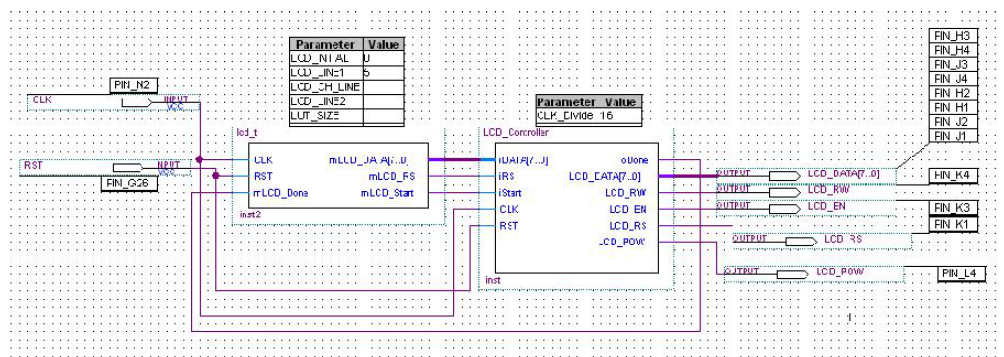
\includegraphics[width=\linewidth]{figures/Exp4_Figure_2.png}
    \captionof{figure}{Schematic diagram for the LCD interface: \texttt{lcd\_t} (lookup-table sequencer) feeding \texttt{LCD\_Controller} (bus-timing controller).}
    \label{fig:exp5-schematic}
  \end{boxedfigure}
  \vspace*{1em
  }
  \begin{boxedtable}
    \captionof{table}{Pin assignment for the LCD interface.}
    \label{tab:exp5-pinassign}
    {\renewcommand{\arraystretch}{1.5}
      \centering
      \begin{tabular}{clcl}
        \toprule
        \# & Node name    & Direction & Location \\
        \midrule
        1  & LCD\_DATA[7] & Output    &          \\
        2  & LCD\_DATA[6] & Output    &          \\
        3  & LCD\_DATA[5] & Output    &          \\
        4  & LCD\_DATA[4] & Output    &          \\
        5  & LCD\_DATA[3] & Output    &          \\
        6  & LCD\_DATA[2] & Output    &          \\
        7  & LCD\_DATA[1] & Output    &          \\
        8  & LCD\_DATA[0] & Output    &          \\
        9  & LCD\_EN      & Output    &          \\
        10 & LCD\_POW     & Output    &          \\
        11 & LCD\_RS      & Output    &          \\
        12 & LCD\_RW      & Output    &          \\
        13 & CLK          & Input     &          \\
        14 & RST          & Input     &          \\
        \bottomrule
      \end{tabular}
    }
  \end{boxedtable}

  \begin{codepanel}{lcd\_t.v --- Appendix 1: lookup-table sequencer (part 1 of 2)}{verilogstyle}
    \begin{lstlisting}
    module lcd_t (
        // Host side
        CLK, RST, mLCD_Done,
        mLCD_DATA, mLCD_RS, mLCD_Start
    );
      // Host side
      input  CLK, RST, mLCD_Done;
      // Internal wires/registers
      output [7:0] mLCD_DATA;
      output mLCD_RS, mLCD_Start;
      reg  [5:0] LUT_INDEX;
      reg  [8:0] LUT_DATA;
      reg  [5:0] mLCD_ST;
      reg  [17:0] mDLY;
      reg  mLCD_Start;
      reg  [7:0] mLCD_DATA;
      reg  mLCD_RS;
      wire mLCD_Done;

      parameter LCD_INITIAL = 0;
      parameter LCD_LINE1   = 5;
      parameter LCD_CH_LINE = LCD_LINE1 + 16;
      parameter LCD_LINE2   = LCD_LINE1 + 16 + 1;
      parameter LUT_SIZE    = LCD_LINE1 + 32 + 1;

      // Sequencing state machine: send one LUT entry, wait for
      // LCD_Controller to finish (mLCD_Done), pause, then advance.
      always @(posedge CLK or negedge RST)
      begin
        if (!RST)
        begin
          LUT_INDEX  <= 0;
          mLCD_ST    <= 0;
          mDLY       <= 0;
          mLCD_Start <= 0;
          mLCD_DATA  <= 0;
          mLCD_RS    <= 0;
        end
        else if (LUT_INDEX < LUT_SIZE)
        begin
          case (mLCD_ST)
            0: begin
              mLCD_DATA  <= LUT_DATA[7:0];
              mLCD_RS    <= LUT_DATA[8];
              mLCD_Start <= 1;
              mLCD_ST    <= 1;
            end
            1: if (mLCD_Done) begin
              mLCD_Start <= 0;
              mLCD_ST    <= 2;
            end
    \end{lstlisting}
  \end{codepanel}

  \begin{codepanel}{lcd\_t.v --- Appendix 1: lookup-table sequencer (part 2 of 2, continued)}{verilogstyle}
    \begin{lstlisting}
            2: if (mDLY < 18'h3FFFE)
                 mDLY <= mDLY + 1;
               else begin
                 mDLY    <= 0;
                 mLCD_ST <= 3;
               end
            3: begin
              LUT_INDEX <= LUT_INDEX + 1;
              mLCD_ST   <= 0;
            end
          endcase
        end
      end
      // Lookup table: LCD_INITIAL entries are setup commands
      // (function set, display on, clear, entry mode, home);
      // LCD_LINE1 / LCD_LINE2 entries are ASCII characters for
      // each line, with the MSB (bit 8) marking RS = 1 (data).
      always
      begin
        case (LUT_INDEX)
          LCD_INITIAL+0: LUT_DATA <= 9'h038;  // function set
          LCD_INITIAL+1: LUT_DATA <= 9'h00C;  // display on
          LCD_INITIAL+2: LUT_DATA <= 9'h001;  // clear display
          LCD_INITIAL+3: LUT_DATA <= 9'h006;  // entry mode set
          LCD_INITIAL+4: LUT_DATA <= 9'h080;  // cursor home, line 1
          // Line 1: "Welcome to the "
          LCD_LINE1+0:  LUT_DATA <= 9'h120;
          LCD_LINE1+1:  LUT_DATA <= 9'h157;
          LCD_LINE1+2:  LUT_DATA <= 9'h165;
          // ... remaining characters follow the same pattern ...
          LCD_LINE1+15: LUT_DATA <= 9'h120;
          LCD_CH_LINE:  LUT_DATA <= 9'h0C0;   // move to line 2
          // Line 2: "    EEM 441 Lab "
          LCD_LINE2+0:  LUT_DATA <= 9'h120;
          LCD_LINE2+4:  LUT_DATA <= 9'h145;
          // ... remaining characters follow the same pattern ...
          LCD_LINE2+15: LUT_DATA <= 9'h120;
          default:      LUT_DATA <= 9'h000;
        endcase
      end
    endmodule
      \end{lstlisting}
  \end{codepanel}
  \vspace{-4pt}
  \listingcaption{lst:exp5-lcdt}{\texttt{lcd\_t.v} --- lookup-table LCD message sequencer.}

  \begin{codepanel}{LCD\_Controller.v --- Appendix 2: bus-timing controller (part 1 of 2)}{verilogstyle}
    \begin{lstlisting}
module LCD_Controller (
    // Host side
    iDATA, iRS, iStart, oDone, CLK, RST,
    // LCD interface
    LCD_DATA, LCD_RW, LCD_EN, LCD_RS, LCD_POW
);
  parameter CLK_Divide = 16;

  // Host side
  input  [7:0] iDATA;
  input  iRS, iStart;
  input  CLK, RST;
  output reg oDone;

  // LCD interface
  output [7:0] LCD_DATA;
  output reg LCD_EN;
  output LCD_RW;
  output LCD_RS;
  output LCD_POW;

  // Internal registers
  reg [4:0] Cont;
  reg [1:0] ST;
  reg preStart, mStart;

  // Write-only interface: bypass iRS straight to LCD_RS
  assign LCD_DATA = iDATA;
  assign LCD_RW   = 1'b0;
  assign LCD_RS   = iRS;
  assign LCD_POW  = 1'b1;
  always @(posedge CLK or negedge RST)
  begin
    if (!RST)
    begin
      oDone    <= 1'b0;
      LCD_EN   <= 1'b0;
      preStart <= 1'b0;
      mStart   <= 1'b0;
      Cont     <= 0;
      ST       <= 0;
    end
    else
    begin
      // Rising-edge detect on iStart
      preStart <= iStart;
      if ({preStart, iStart} == 2'b01)
      begin
        mStart <= 1'b1;
        oDone  <= 1'b0;
      end
\end{lstlisting}
  \end{codepanel}

  \begin{codepanel}{LCD\_Controller.v --- Appendix 2: bus-timing controller (part 2 of 2, continued)}{verilogstyle}
    \begin{lstlisting}
      if (mStart)
      begin
        case (ST)
          0: ST <= 1;                 // wait setup
          1: begin
            LCD_EN <= 1'b1;           // raise enable
            ST     <= 2;
          end
          2: if (Cont < CLK_Divide)   // hold enable pulse width
               Cont <= Cont + 1;
             else
               ST <= 3;
          3: begin
            LCD_EN <= 1'b0;           // drop enable: latches data
            mStart <= 1'b0;
            oDone  <= 1'b1;
            Cont   <= 0;
            ST     <= 0;
          end
        endcase
      end
    end
  end
endmodule
\end{lstlisting}
  \end{codepanel}
  \vspace{-4pt}
  \listingcaption{lst:exp5-lcdctrl}{\texttt{LCD\_Controller.v} --- generates the LCD enable-pulse timing.}

  \textbf{Activity 2 --- Displaying DIP switch input on the LCD}\vspace{2pt}

  \textit{Objective: display the live 8-bit DIP switch configuration on the LCD.}

  \begin{enumerate}
    \item Write Verilog code that reads the 8-bit DIP switch configuration and displays it on the LCD (e.g.\ if switch 1 is turned on, the LCD should display \texttt{1} in the corresponding position).
    \item Print and submit the Verilog code and simulation result.
  \end{enumerate}
  \vspace*{1.5em}

  \begin{introduction}
    Unlike an ordinary DC motor, a stepper motor does not spin freely when power is applied --- it must be driven with a continuously pulsed sequence of specific coil-energising patterns. Each pulse advances the rotor by a fixed step angle (for this motor, $3.6^\circ$ per step), which is what gives stepper motors their positioning precision: as long as speed and torque stay within the motor's limits, the controller always knows the rotor's exact position.
    \vspace*{1.5em}

    The rotor is driven by the interaction of magnetic fields as coils are switched on and off in sequence. Table~\ref{tab:exp6-stepseq} shows the normal four-coil unipolar step sequence; taking a step means driving two of the four coil-driver pins high at a time, in the order shown, through the ULN2003 driver.
  \end{introduction}

  \needspace{4cm}
  \begin{boxedtable}
    \captionof{table}{Normal step sequence for a four-coil unipolar stepper motor.}
    \label{tab:exp6-stepseq}
    {\renewcommand{\arraystretch}{1.5}
      \centering
      \begin{tabular}{lccccc}
        \toprule
        Coil    & Step 1 & Step 2 & Step 3 & Step 4 & Step 1 \\
        \midrule
        1 (B)   & 1      & 1      & 0      & 0      & 1      \\
        2 (\=B) & 0      & 0      & 1      & 1      & 0      \\
        3 (A)   & 1      & 0      & 0      & 1      & 1      \\
        4 (\=A) & 0      & 1      & 1      & 0      & 0      \\
        \bottomrule
      \end{tabular}
    }
  \end{boxedtable}

  \textbf{Activity 3 --- Verilog stepper motor controller}\vspace{2pt}

  \textit{Objective: write Verilog code to control the motion of a stepper motor.}

  \begin{enumerate}
    \item Open Quartus II and start the New Project Wizard.
          \begin{itemize}
            \item Working directory: \texttt{fpga}; project name: \texttt{activity1}; top-level entity: \texttt{step}.
            \item Device family: Cyclone II (\texttt{EP2C35F672C6N}) or Cyclone IV (\texttt{EP4CE115F29C7N}).
            \item Accept the default EDA tool settings and finish.
          \end{itemize}
    \item Create a new Verilog HDL file and enter the code in Listing~\ref{lst:exp6-step} (\texttt{step}, \texttt{divider}, and \texttt{stepper} modules).
    \item Save as \texttt{step} and start compilation.
    \item Use \textbf{Tools} $\to$ \textbf{Netlist Viewer} $\to$ \textbf{RTL Viewer} to generate the block overview shown in Figure~\ref{fig:exp6-rtl}.
    \item Assign pin numbers as shown in Table~\ref{tab:exp6-pins} (refer to the DE2 user manual). For the \texttt{phaseout} outputs that interface with the stepper motor driver, use expansion header \texttt{GPIO\_0}.
    \item Download the program to the Altera DE2 board.
    \item Discuss the result.
  \end{enumerate}

  \begin{boxedfigure}
    \centering
    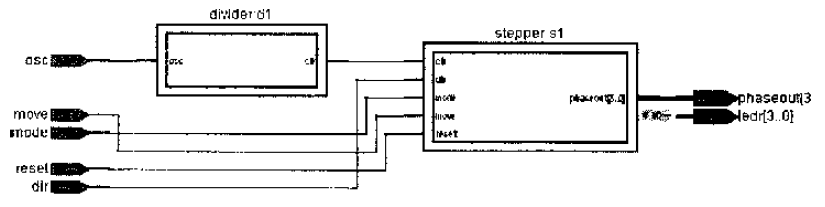
\includegraphics[width=\linewidth]{figures/Exp4_Figure_3.png}
    \captionof{figure}{RTL Viewer overview of the \texttt{step} top-level module.}
    \label{fig:exp6-rtl}
  \end{boxedfigure}

  \begin{boxedtable}
    \captionof{table}{Pin assignment for stepper motor control.}
    \label{tab:exp6-pins}
    {\renewcommand{\arraystretch}{1.5}
      \centering
      \begin{tabular}{cccc|cccc}
        \toprule
        \# & Node name   & Direction & Pin location & \# & Node name   & Direction & Pin location \\
        \midrule
        1  & osc         & Input     &              & 5  & ledr[0]     & Output    &              \\
           & dir (SW0)   & Input     &              & 6  & phaseout[3] & Output    &              \\
           & mode (SW1)  & Input     &              & 7  & phaseout[2] & Output    &              \\
           & move (SW2)  & Input     &              & 8  & phaseout[1] & Output    &              \\
           & reset (SW3) & Input     &              & 9  & phaseout[0] & Output    &              \\
        2  & ledr[3]     & Output    &              &    &             &           &              \\
        3  & ledr[2]     & Output    &              &    &             &           &              \\
        4  & ledr[1]     & Output    &              &    &             &           &              \\
        \bottomrule
      \end{tabular}
    }
  \end{boxedtable}
  \newpage

  \begin{codepanel}{step.v --- top-level module}{verilogstyle}
    \begin{lstlisting}
//============================================================
// Stepper Motor Controller
//============================================================
// TOP LEVEL MODULE
// reset (active low) brings the shaft to its reference position.
// mode selects step (1) or continuous (0) operation.
// dir selects clockwise (1) or anti-clockwise (0) motion.
// move shifts the shaft by one half-step in step mode.
module step(osc, reset, dir, mode, move, phaseout, ledr);
  input  osc, reset, mode, dir, move;
  output [3:0] phaseout, ledr;

  wire clk;

  divider d1 (
    .osc (osc),
    .clk (clk)
  );

  stepper s1 (
    .clk      (clk),
    .reset    (reset),
    .dir      (dir),
    .mode     (mode),
    .move     (move),
    .phaseout (phaseout)
  );
endmodule
\end{lstlisting}
  \end{codepanel}

  \begin{codepanel}{step.v --- motor controller module (part 1 of 2)}{verilogstyle}
    \begin{lstlisting}
// Module stepper is the motor controller.
module stepper(clk, reset, dir, mode, move, phaseout);
  input  clk, reset, dir, mode, move;
  output [3:0] phaseout;
  reg [3:0] phaseout, position, ledr;

  always @(posedge clk or negedge reset)
  begin
    if (reset == 0) begin
      // motor resets to phase 1000 when reset is asserted
      phaseout = 4'b1000;
      ledr     = phaseout;
    end
    else begin
      if (mode == 0) begin
        // Mode = 0: continuous motion.
        // The 8-state sequence below follows Table 1 in both
        // directions; only the first two states are shown here,
        // the remaining six states (0100, 0110, 0010, 0011,
        // 0001, 1001) follow the identical if(dir==0)/else
        // pattern, cycling back to 1000.
        case (phaseout)
          4'b1000: if (dir == 0) begin
            phaseout = 4'b1100;  ledr = phaseout;
          end else begin
            phaseout = 4'b1001;  ledr = phaseout;
          end
          4'b1100: if (dir == 0) begin
            phaseout = 4'b0100;  ledr = phaseout;
          end else begin
            phaseout = 4'b1000;  ledr = phaseout;
          end
          // ... 4'b0100, 4'b0110, 4'b0010, 4'b0011,
          //     4'b0001, 4'b1001 follow the same pattern ...
          default: $display("invalid input");
        endcase
      end
      else begin
        // Mode = 1: single-step motion, advances only when
        // move == 0. Uses the same 8-state sequence as above,
        // indexed by `position` instead of `phaseout`.
        if (move == 1'b0) begin
          case (position)
            // ... identical 8-state sequence as continuous
            //     mode, see Table 1 ...
            default: $display("invalid input");
          endcase
        end
      end
    end
  end
\end{lstlisting}
  \end{codepanel}
  \vspace{-4pt}

  \begin{codepanel}{step.v --- motor controller module (part 2 of 2)}{verilogstyle}
    \begin{lstlisting}
  // Motor advances by one half-step on the falling edge of move.
  always @(negedge move or negedge reset)
  begin
    if (reset == 0) begin
      position = 4'b1000;  // NOTE: corrected from the original
                            // listing, which printed this value
                            // as "4.101011" -- likely a
                            // transcription error; 4'b1000
                            // matches the reset state used
                            // consistently elsewhere.
      ledr = position;
    end
    else if (reset == 1) begin
      position = phaseout;
      ledr     = phaseout;
    end
  end
endmodule
\end{lstlisting}
  \end{codepanel}
  \vspace{-4pt}

  \begin{codepanel}{step.v --- clock divider module}{verilogstyle}
    \begin{lstlisting}
// Module divider divides the incoming clock to produce a
// clock suitable for driving the motor controller.
module divider(osc, clk);
  input  osc;
  output clk;
  reg    clk;
  reg [15:0] count;

  initial count = 16'b0000000000000000;

  always @(posedge osc)
  begin
    count = count + 1;
    clk   = count[15];
  end
endmodule
\end{lstlisting}
  \end{codepanel}
  \vspace{-4pt}
  \listingcaption{lst:exp6-step}{\texttt{step.v} --- top-level, motor-controller, and clock-divider modules.}
  \vspace{1.5em}

  \textbf{Activity 4 --- Variable-speed control with display feedback}\vspace{2pt}

  \textit{Objective: extend the controller with selectable speed and direction/mode feedback.}

  \begin{enumerate}
    \item Write Verilog code that allows selection of three different speeds for the stepper motor in continuous-motion mode.
    \item Display the motor's direction of rotation on the seven-segment display, and the current mode (step / continuous) on the LCD display.
    \item Print and submit the Verilog code and schematic diagram.
  \end{enumerate}

\end{procedure}

\begin{labsection}{Appendix: Stepper Motor Datasheet Reference}{}
  Relevant specifications and wiring information for the Parallax \#27964 stepper motor used in this experiment, extracted from the manufacturer datasheet (see References).
  \begin{boxedfigure}
    \centering
    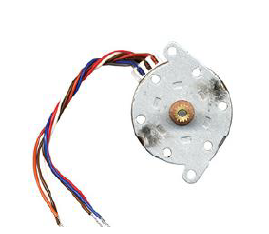
\includegraphics[width=0.8\linewidth]{figures/Exp4_Motor.png}
    \captionof{figure}{Parallax \#27964 stepper motor.}
    \label{fig:exp6-motor}
  \end{boxedfigure}

  \begin{boxedtable}
    \captionof{table}{Technical specifications, Parallax \#27964 stepper motor.}
    \label{tab:exp6-motorspecs}
    {\renewcommand{\arraystretch}{1.4}
      \centering
      \begin{tabular}{|l|c|}
        \hline
        Parameter                        & Value                   \\
        \hline
        Type                             & 4-phase, 12\,V unipolar \\
        \hline
        Step angle                       & $3.6^\circ$ per step    \\
        \hline
        Phase resistance                 & $75\,\Omega$            \\
        \hline
        Current                          & 150\,mA                 \\
        \hline
        Phase inductance                 & 39\,mH                  \\
        \hline
        Detent torque                    & 80\,g$\cdot$cm          \\
        \hline
        Holding torque                   & 600\,g$\cdot$cm         \\
        \hline
        Mounting hole spacing (diagonal) & 1.73\,in                \\
        \hline
        Mounting hole diameter           & 0.11\,in                \\
        \hline
        Shaft diameter                   & 0.197\,in               \\
        \hline
        Shaft length                     & 0.43\,in                \\
        \hline
        Motor diameter                   & 1.66\,in                \\
        \hline
        Motor height                     & 1.35\,in                \\
        \hline
        Weight                           & 0.55\,lb                \\
        \hline
      \end{tabular}
    }
  \end{boxedtable}
  \vspace*{1.5em}

  \begin{boxedfigure}
    \centering
    \begin{tikzpicture}[
        lbl/.style={font=\small},
        % Custom style for the vertical coils matching the image look
        coil style/.style={
            decorate,
            decoration={coil, amplitude=1.5mm, segment length=2.0mm, pre length=1mm, post length=1mm},
            thick
          }
      ]
      % --- Outer Circle ---
      \draw[thick] (0,0) circle (3.2cm);

      % --- Center Common Connection ---
      \node[lbl] at (0,3.9) {{\plexmedium Black}};
      \node[lbl] at (0,3.6) {Common};
      \draw[thick] (0,3.4) -- (0,0); % Vertical common line
      \draw[thick] (-0.8,0) -- (0.8,0); % Horizontal center-tap link

      % --- LEFT SIDE (Phase A) ---
      % Horizontal lead-in lines from outside the circle
      \draw[thick] (-3.8,1.3) -- (-0.8,1.3);   % Top left wire (White)
      \draw[thick] (-3.8,-1.3) -- (-0.8,-1.3); % Bottom left wire (Green)

      % Vertical Coils (Split into two halves to cleanly meet the center tap)
      \draw[coil style] (-0.8,1.3) -- (-0.8,0);
      \draw[coil style] (-0.8,0) -- (-0.8,-1.3);

      % Left Labels
      \node[lbl, anchor=east] at (-3.9,1.3) {B};
      \node[lbl, anchor=south] at (-4.5,1.5) {{\plexmedium Red / Orange}};

      \node[lbl, anchor=east] at (-3.9,-1.3) {$\overline{\text{\=B}}$};
      \node[lbl, anchor=north] at (-4.5,-1.5) {{\plexmedium Brown / Red}};


      % --- RIGHT SIDE (Phase B) ---
      % Horizontal lead-in lines from outside the circle
      \draw[thick] (3.8,1.3) -- (0.8,1.3);   % Top right wire (Brown)
      \draw[thick] (3.8,-1.3) -- (0.8,-1.3); % Bottom right wire (Red)

      % Vertical Coils
      \draw[coil style] (0.8,1.3) -- (0.8,0);
      \draw[coil style] (0.8,0) -- (0.8,-1.3);

      % Right Labels (Matched to image: Brown is B-bar, Red is B)
      \node[lbl, anchor=west] at (3.9,1.3) {$\overline{\text{A}}$};
      \node[lbl, anchor=south] at (4.5,1.5) {{\plexmedium White / Blue}};

      \node[lbl, anchor=west] at (3.9,-1.3) {\=A};
      \node[lbl, anchor=north] at (4.5,-1.5) {{\plexmedium Green / White}};

    \end{tikzpicture}
    \captionof{figure}{Coil winding and lead-wire colours, Parallax \#27964 stepper motor.}
    \label{fig:exp6-coils}
  \end{boxedfigure}

  \begin{boxedfigure}
    \centering
    \begin{tikzpicture}[node distance=8mm and 14mm]
      \node[block, minimum width=2.6cm, minimum height=4.3cm] (drv) {ULN2803\\Darlington\\array};
      \node[io, left=of drv, yshift=1.8cm] (p4) {P4};
      \node[io, left=of drv, yshift=0.55cm] (p5) {P5};
      \node[io, left=of drv, yshift=-0.55cm] (p6) {P6};
      \node[io, left=of drv, yshift=-1.8cm] (p7) {P7};
      \node[io, left=of drv, yshift=-3.0cm] (gnd) {GND};

      \draw[arr] (p4) -- ($(drv.west)+(0,1.8)$);
      \draw[arr] (p5) -- ($(drv.west)+(0,0.55)$);
      \draw[arr] (p6) -- ($(drv.west)+(0,-0.55)$);
      \draw[arr] (p7) -- ($(drv.west)+(0,-1.8)$);
      \draw[arr] (gnd) -| ($(drv.south)+(-0.5,0)$);

      \node[block, right=32mm of drv, minimum width=2.8cm, minimum height=4.3cm] (motor) {Stepper\\Motor\\(\#27964)};
      \node[io, below=6mm of motor] (vcc) {+12\,VDC};
      \draw[arr] (motor.south) -- (vcc);

      \draw[arr] ($(drv.east)+(0,1.8)$)  -- ($(motor.west)+(0,1.8)$)  node[midway, above, font=\scriptsize] {Red};
      \draw[arr] ($(drv.east)+(0,0.55)$) -- ($(motor.west)+(0,0.55)$) node[midway, above, font=\scriptsize] {Brown};
      \draw[arr] ($(drv.east)+(0,-0.55)$) -- ($(motor.west)+(0,-0.55)$) node[midway, below, font=\scriptsize] {White};
      \draw[arr] ($(drv.east)+(0,-1.8)$) -- ($(motor.west)+(0,-1.8)$) node[midway, below, font=\scriptsize] {Green};
      \draw[arr] ($(drv.south)+(0.5,0)$) |- ($(vcc.west)+(-1,0)$) -- (vcc.west) node[pos=-0.92, below, font=\scriptsize] {Black};
    \end{tikzpicture}
    \captionof{figure}{Reference driver-wiring diagram.}
    \label{fig:exp6-driverwiring}
  \end{boxedfigure}

  Note:
  \begin{enumerate}
    \item The P4--P7 labelling above follows the datasheet's original microcontroller example; in this experiment, the corresponding driver inputs are instead the \texttt{phaseout[3:0]} outputs of the \texttt{stepper} module, assigned to DE2 GPIO pins as listed in Table~\ref{tab:exp6-pins}.
    \item The GND are to be common ground with the DE2 board, ULN2803 and the power source.
    \item The +12\,VDC is to be supplied from an external power source, not the DE2 board.
  \end{enumerate}
\end{labsection}

\begin{labsection}{References}{}
  \begin{enumerate}
    \item Altera DE2 User Manual.
    \item \textit{Introduction to Quartus II Software --- Verilog, VHDL, Schematic}, Altera University Program.
    \item \textit{Introduction to Verilog}, Carleton University course notes.
    \item \textit{Stepper Motor Controller Using MAX~II CPLDs}, Altera Application Note AN-488.
    \item Parallax Inc., \textit{4-Phase 12-Volt 75$\,\Omega$ Unipolar Stepper Motor (\#27964)}, technical datasheet.
  \end{enumerate}
\end{labsection}
